% !TeX encoding = UTF-8
% !TeX spellcheck = ca_ES-valencia
% !TeX root = MatCADAlgLin.tex


Podeu trobar el contingut de la part d'ortogonalitat a \cite[Tema 5]{Bret}, i de la part de formes quadràtiques a (\cite[Tema~8]{Bret},\cite[Tema~4]{NaXa}).
\subsection{Ortogonalitat a \texorpdfstring{$\R^n$}{Rn}}
Considerem l'espai vectorial $\R^n$ i recordem el producte escalar definit com: si $\vec u=\smat{u_1\\u_2\\ \vdots\\u_n}$ i $\vec v=\smat{v_1\\v_2\\ \vdots \\ v_n}$ són vectors d'$\R^n$, llavors:
$$
\vec u \cdot \vec v = \vec u^T \vec v=\sum_{i=1}^n u_iv_i \,.
$$
\begin{definicio}
\begin{itemize}
    \item Diem que dos vectors $\vec u$ i $\vec v$ són \emph{ortogonals} si $\vec u\cdot\vec v=0$.
    \item Definim la \emph{longitud d'un vector}:
    $$
    ||\vec u||=\sqrt{\vec u\cdot \vec u}=\sqrt{\sum_{i=1}^n u_i^2}.
    $$
    \item Diem que un vector $\vec u\in\R^n$ és \emph{unitari} si $||\vec u||=1$.
    \item Diem que els vectors $\vec u_1, \dots, \vec u_k$ de $\R^n$ \emph{són ortogonals}\index{ortogonals} si són ortogonals dos a dos, o sigui, si $\vec u_i\cdot\vec u_j=0$ per a tot $i\neq j$.
    \item Diem que els vectors $\vec u_1, \dots, \vec u_k$ de $\R^n$ \emph{són ortonormals}\index{ortonormals} si són unitaris i ortogonals dos a dos, o sigui, si 
    $$\vec u_i\cdot\vec u_j=\left\{ \begin{array}{ll} 1 & \text{si $i=j$} \\ 0 & \text{si $i\neq j$}\end{array}\right.$$
\end{itemize}
\end{definicio}
\begin{observacio}
Podem passar de vectors no nuls $\vec u_1, \dots, \vec u_k$ de $\R^n$ ortogonals a ortonormals dividint cadascun per la seva norma: si $\vec u_1, \dots, \vec u_k$ de $\R^n$ són no nuls, llavors $\frac{\vec u_1}{||\vec u_1||}, \dots, \frac{\vec u_k}{||\vec u_k||}$ són unitaris, i si $\vec u_i\cdot \vec u_j=0$, llavors, $\frac{\vec u_i}{||\vec u_i||}\cdot \frac{\vec u_j}{||\vec u_j||}=\frac{1}{||\vec u_i|| ||\vec u_j||}(\vec u_i\cdot \vec u_j)=0$.
\end{observacio}
\begin{exemple}
La base estàndard d'$\R^n$ formada pels vectors $\vec e_i$ amb un $1$ a la posició $i$ i $0$ a la resta de posicions és una base ortonormal.
\end{exemple}
\begin{lema}
Si els vectors no nuls $\vec u_1, \dots, \vec u_k$ de $\R^n$ són ortogonals, llavors són linealment independents.\\
En particular, si tenim $n$ vectors $\vec u_1, \dots, \vec u_n$ de $\R^n$ ortonormals, formen una base.
\end{lema}
\begin{proof}
Suposem que tenim una combinació lineal dels vectors $\vec u_1, \dots, \vec u_k$ que dóna zero:
$$
0 = \lambda_1 \vec u_1 + \dots + \lambda_n\vec u_n \,.
$$
Llavors, fent el producte escalar per $\vec u_i$ tenim:
\begin{align*}
    0 &  = (\lambda_1 \vec u_1 + \dots + \lambda_n\vec u_n)\cdot \vec u_i= \\
     & = \lambda_1 (\vec u_1 \cdot \vec u_i) + \dots + \lambda_n(\vec u_n\cdot \vec u_i)=\\
     & = \lambda_i ||\vec u_i||^2\quad \text{(tots els altres productes escalars són zero)}
\end{align*}
Per tant, com que $\vec u_i\neq\vec 0$, $\lambda_i=0$ i són linealment independents.

En el cas de tenir $n$ vectors ortonormals, són $n$ vectors ortogonals no nuls, per tant linealment independents i com que la dimensió de $\R^n$ és $n$, són base (Teorema~\ref{teo:baseV}).
\end{proof}


Veurem més endavant com trobar una base ortonormal d'un subespai $V$ de $\R^n$. Suposem però que tenim $[\vec u_1,\ldots,\vec u_k]$ una base ortonormal de $V$, i considerem la \emph{projecció ortogonal}\index{projecció ortogonal} $\proj_V\colon \R^n\rightarrow \R^n$, que envia un vector $\vec v\in \R^n$ al vector $\proj_V(\vec v) = \vec v^\parallel$, on
\[
\vec v^\parallel = (\vec v\cdot \vec u_1)\vec u_1 + \cdots + (\vec v\cdot \vec u_k)\vec u_k \in V.
\]
Observem que $\proj_V\colon \R^n\rightarrow \R^n$ és una aplicació lineal (per les propietats de linealitat del producte escalar). Com que la seva imatge està continguda a $V$ i $\proj_V(\vec u_i) = \vec u_i$, en deduïm que $\Ima(\proj_V)=V$. A més,
\begin{align*}
\Ker(\proj_V) &= \{\vec w\in\R^n ~|~ \vec w^\parallel = 0\}\\
              &= \{\vec w\in\R^n ~|~ \vec w\cdot \vec u_i = 0, \quad i=1,\ldots k\}\\
              &= \{\vec w\in\R^n ~|~ \vec w\cdot \vec v = 0\quad\text{ per a tot }\vec w \in V\}.
\end{align*}
Donarem un nom al nucli de $\proj_V$:

\begin{definicio}
Donat un subespai $V\subseteq \R^n$, el \emph{complement ortogonal}\index{complement ortogonal} de $V$, que escriurem $V^\perp$, és el conjunt
\[
V^\perp = \{\vec w\in \R^n ~|~ \vec w\cdot \vec v = 0\text{ per a tot } \vec v\in V\}.
\]
\end{definicio}

\begin{proposicio}
Sigui $V\subseteq \R^n$ un subespai d'$\R^n$. Aleshores:
\begin{enumerate}[\rm (a)]
    \item $V^\perp$ també és un subespai d'$\R^n$,
    \item $V \cap V^\perp = \{\vec 0\}$,
    \item $\dim(V)+\dim(V^\perp) = n$,
    \item $(V^\perp)^\perp = V$.
\end{enumerate}
\end{proposicio}
\begin{proof}
La primera afirmació es comprova de manera directa, fent servir les propietats del producte escalar.

Per veure la segona, sigui $\vec w\in V\cap V^\perp$. Per tant, $\vec w\cdot\vec w =\| \vec w\|= 0$. Però l'únic vector de longitud $0$ és el vector nul.

Seguidament, observem que $V=\Ima(\proj_V)$ i que $V^\perp = \ker(\proj_V)$. Per tant, per la fórmula del nucli--imatge (Teorema~\ref{teo:ker+ima}) tenim
\[
\dim(\ker\proj_V) + \dim(\Ima\proj_V) = \dim(\R^n)=n,
\]
com volíem veure.

Finalment, per veure que $(V^\perp)^\perp = V$, denotem $W=V^\perp$. Aleshores, si $\vec v\in V$, i $\vec w\in W$, es té que $\vec v\cdot \vec w = 0$, i per tant $\vec v\in W^\perp$. Concloem doncs que $V\subseteq (V^\perp)^\perp$. Però ara observem que $\dim((V^\perp)^\perp) = n - \dim(V^\perp) = n- (n-\dim(V)) = \dim(V)$. Veiem que $(V^\perp)^\perp$ és un subespai que conté $V$ i que té la mateixa dimensió que $V$ i, per tant, ha de coincidir amb $V$.
\end{proof}
\begin{corollari}\label{cor:V+Vper}
Si $V\subseteq\R^n$ és un subespai d'$\R^n$, aleshores $\R^n=V\oplus V^\perp$.
\end{corollari}
\begin{proof}
Per l'apartat (b) de la proposició anterior, la intersecció és buida. Per l'apartat (c), la suma de de les dimensions és $n$. Per tant, si prenem una base $\calb$ de $V$ i una base $\calc$ de $V^\perp$, el conjunt $\calb\cup\calc$ serà linealment independent i tindrà $n$ elements. Per tant, serà base de $\R^n$, que és el que volíem veure.
\end{proof}
D'aquest corol·lari es dedueix que, donat $V$ un subespai d'$\R^n$, tot vector $\vec w\in\R^n$ es pot escriure de forma única com:
\[
\vec w = \vec w^\parallel + \vec w^\perp
\]
amb $\vec w^\parallel \in V$ i $\vec w^\perp \in V^\perp$. A més, tenim que $\vec w^\perp=\proj_{V^\perp}(\vec w)$.

\subsection{El teorema de Pitàgores}
El conegut teorema de Pitàgores es pot formular a $\R^n$. Fixem-nos que el teorema té dues implicacions.
\begin{teorema}
Si $\vec v$ i $\vec w$ són dos vectors d'$\R^n$, aleshores:
\[
\| \vec v + \vec w \|^2 = \|\vec v\|^2 + \|\vec  w\|^2 \iff \vec v \perp \vec w.
\]
\end{teorema}
\begin{proof}
Calculem:
\[
\| \vec v + \vec w\|^2 = (\vec v+\vec w)\cdot (\vec v+\vec w) = \vec v\cdot \vec v + \vec v\cdot \vec w + \vec w\cdot \vec v + \vec w\cdot \vec w=\|\vec v\|^2 + \|\vec w\|^2 +2(\vec v\cdot \vec w). 
\]
Per tant, la igualtat es compleix si i només si $\vec v\cdot \vec w = 0$.
\end{proof}
\begin{corollari}
Sigui $V\subseteq \R^n$ un subespai. Aleshores
\[
\|\proj_V(\vec w)\| \leq \| \vec w\| \text{ per a tot $\vec w\in\R^n$,}
\]
i la desigualtat és una igualtat si i només si $\vec w\in V$.
\end{corollari}
\begin{proof}
Apliquem el teorema anterior a $\vec w^\parallel$ i $\vec w^\perp$ (notem $\vec w = \vec w^\parallel + \vec w^\perp$).
\[
\|\vec w\|^2 = \|\vec w^\parallel\|^2 + \|\vec w^\perp\|^2,
\]
i per tant
\[
\|\proj_V(\vec w)\|^2 \leq \|\vec w\|^2,
\]
amb igualtat si i només si $\|\vec w^\perp\|^2 = 0$, és a dir si i només si $\vec w^\perp = 0$, que és equivalent a $\vec w\in V$.
\end{proof}

Una aplicació d'aquests resultats és una desigualtat molt famosa, coneguda com la \emph{desigualtat de Cauchy--Schwarz}\index{desigualtat de Cauchy--Schwarz}:
\begin{teorema}
Si $\vec v$ i $\vec w$ són vectors de $\R^n$, aleshores
\[
|\vec v\cdot \vec w|\leq \|\vec v\|\|\vec w\|,
\]
amb igualtat si i només si $\vec v$ i $\vec w$ són paral·lels.
\end{teorema}
\begin{proof}
Si $\vec v=\vec 0$, aleshores la desigualtat es compleix trivialment. En cas contrari, considerem el subespai $V=\langle \vec v\rangle$, i apliquem el resultat anterior. Ja havíem vist la fórmula
\[
\proj_V(\vec w) = \frac{\vec w\cdot \vec v}{\|\vec v\|^2} \vec v,
\]
i per tant
\[
\|\proj_V(\vec w)\| = \frac{|\vec w\cdot \vec v|}{\|\vec v\|^2} \|\vec v\|,
\]
i obtenim
\[
\frac{|\vec w\cdot \vec v|}{\|\vec v\|} \leq \|\vec w\|,
\]
que és la desigualtat que busquem un cop passem $\|\vec v\|$ a l'altra banda (i utilitzem que $\vec w\cdot \vec v=\vec v\cdot \vec w$). La igualtat es dóna si i només si $\vec w\in V$, que és equivalent a $\vec v$ essent paral·lel a $\vec w$.
\end{proof}

Observem que si $\vec v$ i $\vec w$ no són zero, aleshores tenim les desigualtats
\[
-1 \leq \frac{\vec v\cdot \vec w}{\|\vec v\|\|\vec w\|}\leq 1.
\]
\begin{definicio}
Donats dos vectors no-nuls $\vec v$ i $\vec w$ d'$\R^n$, \emph{l'angle entre $\vec v$ i $\vec w$}\index{angle entre dos vectors} és
\[
\theta = \arccos\left(\frac{\vec v\cdot \vec w}{\|\vec v\|\|\vec w\|}\right).
\]
\end{definicio}

\subsection{Mètode de Gram-Schmidt}
Aquest mètode permet calcular una base ortonormal d'un subespai de $\R^n$ a partir de projeccions ortogonals. Fixem les notacions següents:
\begin{itemize}
    \item $V\subset \R^n$ un subespai de dimensió $k$ fixat,
    \item $\calb =[\vec v_1, \dots , \vec v_k]$ una base de $V$,
    \item $V_i=\langle \vec v_1, \dots , \vec v_i\rangle \subset V$ el subespai (de dimensió $i$) generat pels $i$ primers vectors de $\calb$. Tenim que $V_1\subset V_2\subset \cdots \subset V_k=V$.
    \item Si $\vec v_i\in\calb$, denotarem per $\vec v_i^\parallel$ la projecció ortogonal de $\vec v_i$ a $V_{i-1}$ i per $\vec v_i^\perp$ el vector  $\vec v_i - \vec v_i^\parallel$, que és ortogonal a $V_{i-1}$.
\end{itemize}
El mètode de Gram-Schmidt\index{Gram-Schmidt} construeix de forma iterativa una base ortonormal a cada $V_i$:
\begin{itemize}
    \item Considerem primer $V_1=\langle \vec v_1 \rangle$, i una base és $\calb_1=[\vec v_1]$. En aquest cas, definim 
    \[\vec u_1=\frac{1}{||\vec v_1||} \vec v_1\]
    i tenim que $\calc_1=[\vec u_1]$ és una base ortonormal de $V_1$.
    \item Considerem ara $V_2=\langle \vec v_1, \vec v_2 \rangle=\langle \vec u_1, \vec v_2 \rangle$. Pel Corol·lari \ref{cor:V+Vper}, $\vec v_2$ es pot escriure de forma única com:
    \[
    \vec v_2 = \vec v_2^\parallel + \vec v_2^\perp
    \]
    amb $\vec v_2^\parallel\in V_1$ i $\vec v_2\perp \in V_1^\perp$. A més, sabem com calcular-los:
    \[
    \vec v_2^\parallel = \proj_{V_1}(\vec v_2)=(\vec v_2 \cdot \vec u_1)\vec u_1
    \]
    i per tant
    \[
    \vec v_2^\perp = \vec v_2 - \vec v_2^\parallel = \vec v_2 - (\vec v_2 \cdot \vec u_1)\vec u_1.
    \]
    Definim $\vec u_2=\frac{1}{||\vec v_2^\perp||}\vec v_2^\perp$, i tenim que $V_2=\langle \vec u_1, \vec u_2\rangle$, amb $\calc_2=[\vec u_1,\vec u_2]$ una base ortonormal.
    \item Suposem ara que ja tenim $\calc_{i-1}=[\vec u_1, \dots, \vec u_{i-1}]$ una base ortonormal de $V_{i-1}$. Considerem $V_i=\langle\vec v_1, \dots, \vec v_{i-1},\vec v_i\rangle=\langle\vec u_1, \dots, \vec u_{i-1},\vec v_i\rangle$, i escrivim:
    \[
    \vec v_i = \vec v_i^\parallel + \vec v_i^\perp
    \]
    amb $\vec v_i^\parallel\in V_{i-1}$ i $\vec v_i\perp \in V_{i-1}^\perp$. Com que els vectors $\vec u_i$ són ortonormals, el càlcul és:
    \[
    \vec v_i^\parallel = \proj_{V_{i-1}}(\vec v_i)=(\vec v_i \cdot \vec u_1)\vec u_1+ \cdots + (\vec v_i \cdot \vec u_{i-1})\vec u_{i-1}
    \]
    i per tant
    \[
    \vec v_i^\perp = \vec v_i - \vec v_i^\parallel = \vec v_i - (\vec v_i \cdot \vec u_1)\vec u_1- \cdots -(\vec v_i \cdot \vec u_{i-1})\vec u_{i-1}.
    \]
    Definim $\vec u_i=\frac{1}{||\vec v_i^\perp||}\vec v_i^\perp$, i tenim que $V_i=\langle \vec u_1, \dots ,\vec u_i\rangle$, amb $\calc_i=[\vec u_1,\dots,\vec u_i]$ una base ortonormal.
\end{itemize}
\begin{exemple}\label{exemple:GramSchmidt}
Considerem $V=\langle \smat{1\\-1\\-1\\1}, \smat{0\\1\\1\\0}\rangle \subset \R^4$ i volem calcular una base ortonormal.

Comencem amb la base $\calb=[\smat{1\\-1\\-1\\1}, \smat{0\\1\\1\\0}]$ i, seguint el procediment, $V_1=\langle \smat{1\\-1\\-1\\1}\rangle$ i tant sols hem de fer-lo unitari:$||\smat{1\\-1\\-1\\1}||=2$ i per tant $V_1=\langle \smat{1\\-1\\-1\\1}\rangle=\langle \smat{1/2\\-1/2\\-1/2\\1/2}\rangle$.

Calculem ara el segon vector:
\[
\vec v_2^\perp = \smat{0\\1\\1\\0} - (\smat{0\\1\\1\\0}\cdot\smat{1/2\\-1/2\\-1/2\\1/2})\smat{1/2\\-1/2\\-1/2\\1/2}= \smat{0\\1\\1\\0}+\smat{1/2\\-1/2\\-1/2\\1/2}=\smat{1/2\\1/2\\1/2\\1/2}.
\]
Llavors $\vec u_2=\frac{1}{||\vec v_2^\perp||} \vec v_2^\perp=\smat{1/2\\1/2\\1/2\\1/2}$.

Tenim, doncs, que $\calc=[\smat{1/2\\-1/2\\-1/2\\1/2},\smat{1/2\\1/2\\1/2\\1/2}]$ és una base ortonormal de $V$.

A més, la matriu del canvi de base és:
\[
S_{\calb,\calc}=\begin{pmatrix} 2 & -1 \\ 0 & 1\end{pmatrix}
\]
\end{exemple}

L'algorisme de Gram-Schmidt ens porta a la factorització $QR$ d'una matriu $A$ (amb les seves columnes linealment independents).
\begin{teorema}
Donada una matriu $A\in M_{m\times n}(\R)$ amb les seves columnes linealment independents, existeixen una matriu $Q\in M_{m\times n}(\R)$ i $R\in M_{n\times n}$ tals que:
\begin{itemize}
    \item $A=QR$,
    \item $Q^T Q=\1_n$ (diem que $Q$ és una matriu ortogonal\index{matriu!ortogonal}),
    \item $R$ és una matriu triangular superior amb els coeficients de la diagonal positius.
\end{itemize}
A més, aquesta factorització és única.
\end{teorema}
\begin{proof}
La demostració és constructiva: anirem calculant els coeficients de les columnes $Q$ i $R$ aplicant el mètode de Gram-Schmidt. Fixem abans les notacions següents per a les columnes d'$A$, de $Q$ i els coeficients de $R$:
\[
A=\begin{pmatrix} | & | & & | \\ \vec v_1 & \vec v_2 & \cdots & \vec v_n \\ | & | & & | \end{pmatrix} ,
Q=\begin{pmatrix} | & | & & | \\ \vec u_1 & \vec u_2 & \cdots & \vec u_n \\ | & | & & | \end{pmatrix} 
\text{ i }
R=\begin{pmatrix} r_{11} & r_{12} & \cdots & r_{1n} \\ 0 & r_{22} & \cdots & r_{2n} \\ \vdots & \vdots & \ddots & \vdots \\ 0 & 0 & \cdots & r_{nn}\end{pmatrix}.
\]
I les matrius formades per les primeres $j$ columnes d'$A$, $Q$ i la submatriu quadrada $j\times j$ d'$R$:
\[
A_j=\begin{pmatrix} | & | & & | \\ \vec v_1 & \vec v_2 & \cdots & \vec v_j\\ | & | & & | \end{pmatrix} ,
Q_j=\begin{pmatrix} | & | & & | \\ \vec u_1 & \vec u_2 & \cdots & \vec u_j \\ | & | & & | \end{pmatrix} 
\text{ i }
R_j=\begin{pmatrix} r_{11} & r_{12} & \cdots & r_{1j} \\ 0 & r_{22} & \cdots & r_{2j} \\ \vdots & \vdots & \ddots & \vdots \\ 0 & 0 & \cdots & r_{jj}\end{pmatrix}.
\]
La construcció comença amb $j=1$, $j=2$ i veurem com es fa el cas $j$ a partir del $j-1$:
\begin{itemize}
    \item Cas $j=1$: llavors $A_1=\vec v_1$: calculem el coeficient $R_1=(r_{11})=(||\vec v_1||)$ i la primera columna de $Q$ com $Q_1=\vec u_1=\frac{1}{r_{11}}\vec v_1$. Veiem que, de moment, es compleix  $A_1=Q_1R_1$. A més, $Q_1^TQ_1=||\vec u_1||=1$ i $R_1$ és triangular superior i amb la diagonal positiva (és un mòdul).
    \item Cas $j=2$: considerem $r_{12}=\vec u_1\cdot \vec v_2$, el vector $\vec v_2^\perp=\vec v_2-r_{12}u_1$, $r_{22}=||\vec v_2^\perp||$ i $\vec u_2=\frac{1}{r_{22}} v_2^\perp$. La primera columna de $Q_2R_2$ és la mateixa que la de $Q_1R_1=A_1$. La segona és
    \[
    r_{12}u_1+r_{22}\vec u_2=(u_1\cdot v_2)\vec u_1+||v_2-(\vec u_1\cdot \vec v_2)\vec u_1||\frac{1}{||\vec v_2-(\vec u_1\cdot \vec v_2)\vec u_1||}(\vec v_2-(\vec u_1\cdot \vec v_2)\vec u_1)=\vec v_2
    \]
    i per tant tenim la segona columna de $A$, llavors $A_2=Q_2R_2$. També veiem que $Q_2^TQ_2=\1_2$ ($u_2$ és perpendicular a $\vec u_1$ i tots dos són unitaris) i $R_2$ és triangular superior i la diagonal positiva (són mòduls de vectors).
    \item Suposem que tenim les $j-1$ primeres columnes de $Q$, i les de $R$ tal que $A_{j-1}=Q_{j-1}R_{j-1}$, $Q_{j-1}^TQ_{j-1}=\1_{j-1}$ i $R_{j-1}$ triangular superior i amb la diagonal positiva. Considerem $r_{ij}=\vec u_i\cdot \vec v_j$ per a $1\leq i <j$, $\vec v_j^\perp=\vec v_j-r_{1j}\vec u_1-\cdots-r_{(j-1)j}\vec u_{j-1}$, $r_{jj}=||\vec v_j^\perp||$ i $\vec u_j=\frac{1}{r_{jj}} \vec v_j^\perp$. Si fem $Q_jR_j$, les primeres $j-1$ columnes són les de $Q_{j-1}R_{j-1}$, per tant són $A_{j-1}$. Si calculem la columna $j$-èssima de $Q_jR_j$:
    \begin{align*}
     r_{1j}\vec u_1+\cdots+r_{jj}\vec u_j & =(\vec u_1\cdot \vec v_j)\vec u_1+\cdots+(\vec u_{j-1}\cdot \vec v_j)\vec u_{j-1}+||\vec v_j^\perp||\frac{1}{||\vec v_j^\perp||} \vec v_j^\perp = \\
     & =(\vec u_1\cdot \vec v_j)\vec u_1+\cdots+(\vec u_{j-1}\cdot \vec v_j)\vec u_{j-1}+ \vec v_j^\perp=\vec v_j .
    \end{align*}
    I per tant $A_j=Q_jR_j$. A més, la primera caixa $(j-1)\times(j-1)$ superior esquerra de $Q_j^TQ_j$ és una $\1_{j-1}$. L'última columna i fila són és $\vec u_i\cdot \vec u_j$, i per tant, com que $\vec u_j$ és perpendicular als altres $\vec u_i$ i unitari, tenim que $Q_j^TQ_j=\1_j$. Finalment, $R_j$ és triangular superior per construcció, i la diagonal formada per mòduls, per tant positius.
\end{itemize}
Falta veure la unicitat, també per inducció sobre $j$:
\begin{itemize}
    \item Cas $j=1$: com que $R$ és triangular superior, $v_1=r_{11}\vec u_1$ amb $||\vec u_1||=1$, per tant $\vec u_1=\frac{\pm1}{||\vec v_1||}v_1$, però com que $r_{11}$ és positiva positiva, $\vec u_1=\frac{1}{||\vec v_1||}\vec v_1$ i $r_{11}=||\vec v_1||$.
    \item Suposem que les $j-1$ primeres columnes de $Q$ i de $R$ ja estan fixades, volem veure que tant sols hi ha una elecció per la $j$-èssima: el vector $\vec u_j$ és un vector perpendicular a l'espai $V_{j-1}=\langle \vec v_1, \dots, \vec v_{j-1}\rangle$ i contingut a $V_j=\langle \vec v_1, \dots, \vec v_j\rangle$. Considerem $V_{j-1}^\perp$ el complement ortogonal de $V_{j-1}$ a $V_j$, que és de dimensió $1$ ($\dim(V_{j-1})+\dim(V_{j-1}^\perp)=\dim(V_j)$), i conté $\vec v_j^\perp$, per tant es té $V_{j-1}^\perp=\langle v_j^\perp \rangle$. Llavors, com que ha de ser unitari, ja $j$-èssima columna de $Q$ ha de ser $\vec u_j=\frac{\pm1}{||\vec v_j^\perp||}\vec v_j^\perp$, però com que $r_{jj}$ és positiva positiva, $\vec u_j=\frac{1}{||\vec v_j^\perp||}\vec v_j^\perp$ i $r_{jj}=||\vec v_j^\perp||$, i tenim la unicitat de la $\vec u_j$ i el coeficient $r_{jj}$. La resta de coeficients de la columna $j$ d'$R$ estan determinats per ser $R$ triangular superior (per tant, per sota de $r_{jj}$ són zero) i el fet de que els de sobre són les coordenades de $\vec v_j-\vec v_j^\perp$ en la base $[\vec u_1,\dots,\vec u_{j-1}]$ de $V_{j-1}$ (i les coordenades en una base són úniques pel Teorema~\ref{teo:base_coord_uniq}).
\end{itemize}
\end{proof}
\begin{exemple}
Podem aprofitar els càlculs fets a l'Exemple \ref{exemple:GramSchmidt} per trobar la factorització $QR$ següent:
\[
\begin{pmatrix}
1 & 0 \\ -1 & 1 \\ -1 & 1 \\ 1 & 0
\end{pmatrix}=
\begin{pmatrix}
1/2 & 1/2 \\ -1/2/ & 1/2 \\ -1/2 & 1/2 \\ 1/2 & 1/2
\end{pmatrix}
\begin{pmatrix}
2 & -1 \\ 0 & 1
\end{pmatrix}.
\]
\end{exemple}

\subsection{Aplicacions i matrius ortogonals}
%Conserva normes \iif conserva producte escalar \iif Q^TQ=\id
\begin{definicio}
Diem que una aplicació lineal $f \colon \R^n\to \R^m$ és \emph{ortogonal}\index{aplicació!ortogonal} si conserva la longitud dels vectors, o sigui, si
\[
||f(\vec v)||=||\vec v|| \text{ per a tot $\vec v\in\R^n$.}
\]
Si $f=f_A$ amb $A\in M_{m\times n}(\R)$, direm que $A$ és una \emph{matriu ortogonal}\index{matriu!ortogonal}.
\end{definicio}

\begin{exemple}
Les rotacions definides a la Secció \ref{subsubsec:rotacio} són ortogonals: es pot interpretar geomètricament o bé fent els càlculs: un vector $\smat{x\\y}$ té norma
\[
||\begin{pmatrix}x \\ y \end{pmatrix}||^2=\begin{pmatrix} x & y \end{pmatrix}\begin{pmatrix} x \\ y \end{pmatrix} = x^2+y^2
\]
i va a parar a:
\[
\begin{pmatrix*}[r]
\cos\theta&-\sin\theta\\
\sin\theta&\cos\theta
\end{pmatrix*}
\begin{pmatrix}x \\ y \end{pmatrix} ,
\]
que té norma
\begin{align*}
||f(\smat{x\\y})||^2 & =\left( \begin{pmatrix*}[r]
\cos\theta&-\sin\theta\\
\sin\theta&\cos\theta
\end{pmatrix*}
\begin{pmatrix}x \\ y \end{pmatrix}  \right)^T
\begin{pmatrix*}[r]
\cos\theta&-\sin\theta\\
\sin\theta&\cos\theta
\end{pmatrix*}
\begin{pmatrix}x \\ y \end{pmatrix} = \\
& = \begin{pmatrix}x &  y \end{pmatrix}
\begin{pmatrix*}[r]
\cos\theta&\sin\theta\\
-\sin\theta&\cos\theta
\end{pmatrix*}
\begin{pmatrix*}[r]
\cos\theta&-\sin\theta\\
\sin\theta&\cos\theta
\end{pmatrix*}
\begin{pmatrix}x \\ y \end{pmatrix} = \\
& = \begin{pmatrix}x &  y \end{pmatrix}
\begin{pmatrix*}[r]
1&0\\
0&1
\end{pmatrix*}
\begin{pmatrix}x \\ y \end{pmatrix} = x^2+y^2\\
\end{align*} 
i per tant la rotació és ortogonal.
\end{exemple}
\begin{exercici}
Demostreu ques reflexions definies a la Secció \ref{subsubsec:reflexio} són ortogonals.
\end{exercici}
\begin{exemple}
Les projeccions a un subespai $V\subset \R^n$ ($V\neq \R^n)$ no són ortogonals: considerem $\vec 0 \neq \vec u \in V^\perp$, llavors $\proj_V(\vec u)=\vec 0$ i per tant no es conserva la longitud de $\vec u$.
\end{exemple}

El lema següent ens permet calcular el producte escalar en funció dels mòduls:
\begin{lema}\label{lema:prod_esc_modul}
Si $\vec u, \vec v$ són vectors d'$\R^n$, llavors:
\[
\vec u \cdot \vec v = \frac{1}{2}\left(||\vec u + \vec v||^2 - ||\vec u||^2 - ||\vec v||^2\right).
\]
\end{lema}
\begin{proof}
Considerem $\vec u, \vec v \in \R^n$. Tenim que:
\begin{align*}
||\vec u + \vec v||^2 & =(\vec u+\vec v)\cdot(\vec u+\vec v) = \vec u \cdot (\vec u+ \vec v) + \vec v \cdot (\vec u+ \vec v) = \\
 & = \vec u \cdot \vec u  + \vec u \cdot \vec v + \vec v \cdot \vec u+\vec v \cdot \vec v = ||\vec u||^2+2 (\vec u \cdot \vec v) + ||\vec v||^2
\end{align*}
I per tant:
\[
\vec u \cdot \vec v = \frac{1}{2}\left(||\vec u + \vec v||^2 - ||\vec u||^2 - ||\vec v||^2\right).
\]
\end{proof}
I d'aquí deduïm:
%\begin{teorema}[Pitàgores]\index{Teorema de Pitàgores}
%Els vectors $\vec u$ i $\vec v$ d'$\R^n$ són ortogonals si i només si
%\[
%||\vec u+\vec v||^2 = ||\vec u||^2+||\vec v||^2 .
%\]
%\end{teorema}
%\begin{proof}
%Es dedueix de la igualtat del Lema \ref{lema:prod_esc_modul}.
%\end{proof}
\begin{teorema}
Una aplicació lineal $f\colon \R^n \to \R^m$ és ortogonal si i només si $f(\vec u)\cdot f(\vec v)=\vec u \cdot \vec v$ per a tot $\vec u$ i $\vec v$ de $\R^n$.
\end{teorema}
\begin{proof}
Si l'aplicació és ortogonal, es compleix que, per a tot $\vec u,\vec v \in \R^n$, $||f(\vec u)||=||\vec u||$ i $||f(\vec v)||=||\vec v||$. Llavors:
\begin{align*}
    f(\vec u)\cdot f\vec v) & = \frac{1}{2}\left(||f(\vec u) +f(\vec v)||^2 - ||f(\vec u)||^2 - ||f(\vec v)||^2\right) = \\
    & = \frac{1}{2}\left(||f(\vec u+\vec v)||^2 - ||f(\vec u)||^2 - ||f(\vec v)||^2\right) = \\
     & = \frac{1}{2}\left(||\vec u + \vec v||^2 - ||\vec u||^2 - ||\vec v||^2\right) = \vec u \cdot \vec v  ,
\end{align*}
on hem utilitzat el Lema \ref{lema:prod_esc_modul} dues vegades i que $f$ és lineal.

Si $f(\vec u)\cdot f(\vec v)=\vec u \cdot \vec v$ per a tot $\vec u$ i $\vec v$ de $\R^n$, com que $||\vec u||^2=\vec u \cdot \vec u$, tenim que, agafant $\vec u=\vec v$, $||f(\vec u)||^2=||\vec u||^2$ i per tant $f$ és ortogonal.
\end{proof}
\begin{corollari}
Si $f = f_A \colon \R^n \to \R^m$ és una aplicació lineal i $\vec e_1, \dots, \vec e_n$ és la base estàndard d'$\R^n$, llavors:
\begin{enumerate}[\rm (a)]
    \item $f$ és ortogonal si i només si $f(\vec e_1), \dots, f(\vec e_n)$ són vectors ortonormals. En particular, si $f$ és ortogonal, $f(\vec e_1), \dots, f(\vec e_n)$ són linealment independents i si $n=m$, són una base ortonormal.
    \item $f_A$ és una aplicació lineal ortogonal si i només si $A$ és una matriu ortogonal.
\end{enumerate}
\end{corollari}
\begin{proof}
Vegem primer (a). Si $f$ és ortogonal, del fet que $f(\vec e_i)\cdot f(\vec e_j)=\vec e_i\cdot \vec e_j$, es dedueix que $f(\vec e_i)$ són unitaris i ortogonals dos a dos, per tant, ortonormals.

Suposem ara que $f(\vec e_i)$ són unitaris i ortogonals dos a dos i unitaris i $\vec u \in \R^n$. Tenim que existeixen nombres reals $\lambda_i$ tals que $\vec u= \lambda_1\vec e_1+ \cdots + \lambda_n\vec e_n$. Llavors $||u||^2=\lambda_1^2+ \cdots + \lambda_n^2$, i $||f(\vec u)||^2=||\lambda_1 f(\vec e_1)+\cdots + \lambda_n f(\vec e_n)||^2=\lambda_1^2+ \cdots + \lambda_n^2$ (pel Teorema de Pitàgores, utilitzant que són ortogonals i unitaris). 

Vegem ara que els $f(\vec e_1)$ són linealment independents: més en general, tenim que si $\vec u_1, \dots, \vec u_k$ són vectors ortonormals, llavors són linealment independents: del teorema de Pitàgores es dedueix que:
\[
||\lambda_1\vec u_1 + \cdots + \lambda_k \vec u_k||^2=\lambda_1^2 + \cdots + \lambda_k^2
\]
I per tant si tenim una combinació $\vec 0 = \lambda_1\vec u_1 + \cdots + \lambda_k \vec u_k$, tots els $\lambda$ han de ser zero. Llavors tenim que, en el nostre cas, $f(\vec e_1), \dots, f(\vec e_n)$ són linealment independents.

Si $n=m$, $f(\vec e_1)$, \ldots, $f(\vec e_m)$ són $m$ vectors de $\R^m$ linealment independents, i per tant, base.

Per a veure (b), si $f_A$ és ortogonal i fem el producte $A^TA$, tenim que el coeficient $(i,j)$ és $f(\vec e_i)\cdot f(\vec e_j)$, per tant, com que són ortonormals, tenim $A^TA=\1_n$.

Les columnes d'$A$ són els vectors $f(\vec e_j)$, per tant, $A^TA=\1_n$ si i només si  $f(\vec e_1), \dots, f(\vec e_n)$ són ortogonals i unitaris (per tant $f$ és ortogonal).
\end{proof}
\begin{teorema}
Si $A,B \in M_n(\R)$ són matrius ortogonals, llavors:
\begin{enumerate}[\rm (a)]
    \item $AB$ també és ortogonal i
    \item $A^{-1}$ és ortogonal (i $A^{-1}=A^T)$.
\end{enumerate}
\end{teorema}
\begin{proof}
$AB$ serà ortogonal si $f_{AB}$ conserva la longitud dels vectors, però $f_{AB}=f_A \circ f_B$ i, per hipòtesi, tant $f_B$ com $f_A$ conserven la longitud, per tant, $f_{AB}$ també.

Per a veure (b): si $\vec v = f_{A^{-1}}(\vec w))$, llavors $\vec w=f_A(\vec v)$ i, per hipòtesi $||\vec w||=||f_A(\vec v)||=||\vec v||$, per tant $A^{-1}$ és ortogonal. 
\end{proof}

\subsection{Matriu d'una projecció ortogonal en una base ortonormal}
\begin{proposicio}
Si $V\subset \R^n$ un subespai vectorial, $[\vec v_1, \dots, \vec v_k]$ és una base ortonormal de $V$ i $Q$ és la matriu que té per columnes els vectors $\vec v_j$, llavors, la matriu de la projecció ortogonal a $V$ és:
\[
[\proj_V]=Q Q^T.
\]
\end{proposicio}
 \begin{proof}
 Com que $[\vec v_1, \dots, \vec v_k]$ és una base ortonormal de $V$, la projecció ortogonal a $V$ del vector $\vec u$ és:
 %\[
 %\vec u = \begin{pmatrix}
 %\lambda_1 \\ \vdots \\ \lambda_n
 %\end{pmatrix}
 %\]
 %és
 \[
 \proj_V(\vec u)=(\vec u\cdot \vec v_1)\vec v_1 + \cdots + (\vec u\cdot \vec v_k)\vec v_k = Q \begin{pmatrix}
 \vec u\cdot \vec v_1 \\ \vdots \\ \vec u\cdot \vec v_k \end{pmatrix}= Q \begin{pmatrix}
 \vec v_1^T \vec u \\ \vdots \\ \vec v_k^T \vec u
 \end{pmatrix} = Q
 \begin{pmatrix}
 \vec v_1^T \\
 \vdots \\
 \vec v_k^T
 \end{pmatrix} \vec u
 =(QQ^T)\vec u
 \]
 I per tant la matriu associada a la projecció és $QQ^T$.
 \end{proof}
\begin{exemple}
Considerem el vector $\smat{x\\y}\neq\smat{0\\0}$ de $\R^2$ i calculem la matriu de la projecció a $V=\langle \smat{x\\y}\rangle$. Una base ortonormal és $\vec v_1=\frac{1}{\sqrt{x^2+y^2}}\smat{x\\y}$ i per tan la matriu és (compareu-ho amb la Proposició \ref{prop:projR2}):
\[
[\proj_V]=\frac{1}{\sqrt{x^2+y^2}} \begin{pmatrix} x \\ y \end{pmatrix} \frac{1}{\sqrt{x^2+y^2}} \begin{pmatrix} x & y \end{pmatrix} = \frac{1}{x^2+y^2} \begin{pmatrix} x^2 & xy \\ xy & y^2 \end{pmatrix} .
\]
\end{exemple}
\begin{exemple}
Volem calcular la matriu de la projecció ortogonal de $\R^4$ a $V=\langle \smat{1\\-1\\-1\\1}, \smat{0\\1\\1\\0}\rangle \subset \R^4$. A l'Exemple \ref{exemple:GramSchmidt} ja hem calcular una base ortonormal, i era  $\calc=[\smat{1/2\\-1/2\\-1/2\\1/2},\smat{1/2\\1/2\\1/2\\1/2}]$, per tant la matriu corresponent a la projecció ortogonal és:
\[
\begin{pmatrix}
1/2 & 1/2 \\ -1/2 & 1/2 \\ -1/2 & 1/2 \\ 1/2 & 1/2
\end{pmatrix}
\begin{pmatrix}
1/2 & -1/2 & -1/2 & 1/2 \\ 1/2 & 1/2 & 1/2 & 1/2 
\end{pmatrix}
\begin{pmatrix}
1/2 & 0 & 0 & 1/2 \\
0 & 1/2 & 1/2 & 0 \\
0 & 1/2 & 1/2 & 0 \\
1/2 & 0 & 0 & 1/2
\end{pmatrix}.
\]
\end{exemple}

\subsection{Mínims quadrats}
Aquesta secció suposarem que tenim un conjunt $E$ i un subconjunt $V\subset E$ i que, a cada element d'$E$, volem assignar-li l'element de $V$ que millor l'aproxima. Per això, suposem que $E$ és un $\R$-espai vectorial i que $V$ és un subespai. Llavors:
\begin{proposicio}\label{prop:proj_com_aprox}
Si $E$ és un $\R$-espai vectorial i $V \subset E$ és un subespai, llavors, per a tot $\vec u \in E$ i $\vec v\in V$ es compleix:
\[
||\vec u - \proj_V(u)|| \leq ||\vec u - \vec v||.
\]
\end{proposicio}
\begin{proof}
Tenim que $\vec u - \vec v = (\vec u - \proj_V(u)) + (\proj_V(u) - \vec v)$ amb el primer vector de $\vec V^\perp$ i el segon de $V$. Aplicant el Teorema de Pitàgores tenim:
\[
||\vec u - \vec v||^2= ||\vec u - \proj_V(\vec u)||^2 + ||\proj_V(\vec u) - \vec v||^2 \geq ||\vec u - \proj_V(\vec u)||^2 ,
\]
i tenim la desigualtat que volem.
\end{proof}
Per tant, considerant la mètrica de la distància, la millor aproximació en aquest cas és la projecció ortogonal.

\subsubsection{Recta de regressió}\index{recta de regressió}
Suposem que tenim un núvol de punts  $(x_1,y_1), \dots , (x_k,y_k)$ de $\R^2$ que, en principi, no estan alineats. Suposem, a més, que hi ha una dependència del tipus $y=f(x)$ (per tant, al núvol de punts seria un problema que hi hagués dos punts amb la mateixa $x$ i diferents $y$). Suposem que els punts estan \emph{aproximadament} alineats i que el que volem trobar és la recta $y=a_0+a_1x$ que aproxima millor aquests punts. 

Una altra manera de pensar-ho és que volem resoldre el sistema d'equacions amb incògnites $a_0$ i $a_1$:
\begin{align*}
a_ 0 + x_1 a_1 & = y_1 \\ & \vdots  \\ a_0 + x_k a_k & = y_k 
\end{align*}
O, en forma matricial:
\[
\begin{pmatrix} 1 & x_1 \\ \vdots & \vdots \\ 1 & x_k \end{pmatrix}
\begin{pmatrix} a_0 \\ a_1 \end{pmatrix} =
\begin{pmatrix} y_1 \\ \vdots \\ y_k \end{pmatrix}
\]
Com que molt probablement els punts no estan alineats, com a sistema d'equacions, és un sistema incompatible. Dit d'una altra manera, el vector $\vec y=\smat{y_1 \\ \vdots \\ y_k}$ no pertany al subespai $V=\langle \smat{1 \\ \vdots \\ 1} , \smat{x_1 \\ \vdots \\ x_k} \rangle$. Si apliquem la Proposició \ref{prop:proj_com_aprox}, el vector de $V$ que serà més proper a $\vec y$ serà $\proj_V(\vec y)$:
\[
\proj_V(\begin{pmatrix} y_1 \\ \vdots \\ y_k \end{pmatrix})= a_0 \begin{pmatrix} 1 \\ \vdots \\ 1 \end{pmatrix} + a_1 \begin{pmatrix} x_1 \\ \vdots \\ x_k \end{pmatrix}= \begin{pmatrix} 1 & x_1 \\ \vdots & \vdots \\ 1 & x_k \end{pmatrix}
\begin{pmatrix} a_0 \\ a_1 \end{pmatrix} .
\]
Podríem calcular $a_0$ i $a_1$ fent primer Gram-Schmidt per a trobar una base ortonormal de $V$ i fent els productes escalars corresponents, o bé fent les consideracions següents: el vector
\[
\begin{pmatrix} y_1 \\ \vdots \\ y_k \end{pmatrix} -
\begin{pmatrix} 1 & x_1 \\ \vdots & \vdots \\ 1 & x_k \end{pmatrix}
\begin{pmatrix} a_0 \\ a_1 \end{pmatrix}
\]
és perpendicular a $V$, per tant ha de complir que:
\[
\begin{pmatrix}
1 & \dots & 1 & \\ x_1 & \dots & x_n
\end{pmatrix}
\left(
\begin{pmatrix} y_1 \\ \vdots \\ y_k \end{pmatrix} -
\begin{pmatrix} 1 & x_1 \\ \vdots & \vdots \\ 1 & x_k \end{pmatrix}
\begin{pmatrix} a_0 \\ a_1 \end{pmatrix}\right) = \begin{pmatrix} 0 \\ 0 \end{pmatrix} 
\]
I per tant:
\[
\begin{pmatrix}
1 & \dots & 1 & \\ x_1 & \dots & x_n
\end{pmatrix}
\begin{pmatrix} 1 & x_1 \\ \vdots & \vdots \\ 1 & x_k \end{pmatrix}
\begin{pmatrix} a_0 \\ a_1 \end{pmatrix} = 
\begin{pmatrix}
1 & \dots & 1 & \\ x_1 & \dots & x_k
\end{pmatrix}
\begin{pmatrix} y_1 \\ \vdots \\ y_k \end{pmatrix}
\]
I queda el sistema compatible determinat:
\[
\begin{pmatrix}
k & \sum x_i \\ \sum x_i & \sum x_i^2 
\end{pmatrix}
\begin{pmatrix} a_0 \\ a_1 \end{pmatrix} = 
\begin{pmatrix} \sum y_i \\ \sum x_iy_i \end{pmatrix}
\]
Que es pot escriure: si $\overline x = \frac{1}{k} \sum x_i$, $\overline y=\frac{1}{k} \sum y_i$, $\overline {x^2}= \frac{1}{k} \sum x_i^2$ i $\overline {xy}=  \frac{1}{k} \sum x_iy_i$:
\[
\begin{pmatrix}
1 & \overline x \\ \overline x & \overline{x^2} 
\end{pmatrix}
\begin{pmatrix} a_0 \\ a_1 \end{pmatrix} = 
\begin{pmatrix}  \overline y \\ \overline{xy} \end{pmatrix}
\]
I la solució es pot escriure com:
\begin{equation}\label{eq:recta_reg}
a_1=\frac{\overline{xy} - \overline x \, \overline y}{\overline{x^2} - (\overline x)^2}
\text{ i } 
a_0= \overline y - a_1 \overline x .
\end{equation}
\begin{exemple}
Considerem les notes següents d'un grup de $21$ alumnes corresponent a una avaluació parcial i la nota final que van treure:
\[
\begin{array}{|c|c||c|c||c|c|}
\hline\text{Parcial} & \text{Final} & \text{Parcial} & \text{Final} & \text{Parcial} & \text{Final}  \\ \hline
8.15 & 8.995 & 6.25 & 7.845 & 2.2 & 4.58 \\
0.3 & 1.98 & 5.85 & 7.075 & 4.6 &4.95 \\
4.3&5.01 & 3.55 & 5.715 & 4.7 & 7.08\\
1.8&2.88 & 1.7 & 2.82 & 2.3 & 3.86\\
5.4&5.08 & 4.6 & 7.13 & 2.7 &5.33 \\
0.2 &2.78 & 7.7 & 8.8 & 7.95 &8.595\\
5.4 & 7.77 & 3.15 &1.245 & 3 &4.95\\ \hline
\end{array}
\]
I volem aproximar la nota final a partir de la del parcial amb una recta:
\[
\text{final}= a_0 + a_1 \text{parcial}
\]
Per tant, podem aplicar la Fórmula \eqref{eq:recta_reg} als valors (aproximem a 3 decimals):
\[
\overline{x}=\overline{\text{parcial}}= 4.085, \quad
\overline{y}=\overline{\text{final}}= 5.451, \quad
\overline{x^2}=21,839 \text{ i }
\overline{xy}= 26,816.
\]
I queda (amb 3 decimals):
\[
\text{final}= 1.843 + 0.883 \text{parcial}.
\]
La Figura \ref{fig:recta_reg} té una representació gràfica d'aquestes dades i de la recta de regressió. A més, l'equació de la recta es pot utilitzar per aproximar una nota final a partir d'una parcial: per exemple, un alumne que hagi tret un $4$ al parcial, la predicció diria que trauria un $5,376$ a la nota final.
\begin{figure}[ht]
\center{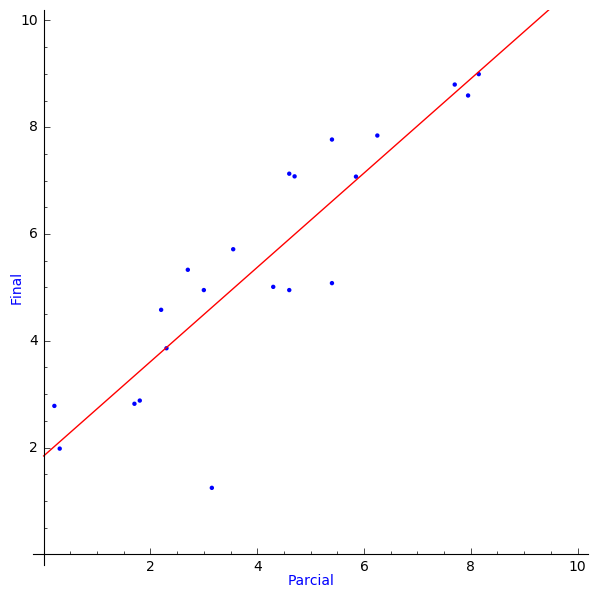
\includegraphics[width=10cm]{regre.png}}
\caption{Recta de regressió\label{fig:recta_reg}}
\end{figure}
\end{exemple}
\subsubsection{Cas general}
En el cas general, suposem que tenim un sistema d'equacions lineals:
\[
A x = b
\]
amb $A\in M_{m\times n}(\R)$ amb $m\geq n$ (més equacions que incògnites) i tal que $\Rang(A)=n$. És molt probable que aquest sistema no tingui solució, i per aquests casos ens interessa tenir la millor aproximació:
\begin{lema}
Amb les hipòtesis anteriors, el sistema
\[
A^T A x = A^T b
\]
té solució única. Aquesta solució s'anomena \emph{solució per mínim quadrats del sistema $Ax=b$}\index{mínims quadrats}.
\end{lema}
\begin{proof}
Observem que $A^TA \in M_{n\times n}(\R)$, pel que tant sols cal veure que $\Rang(A^T A)=n$ (i llavors serà un sistema compatible determinat), o el que és el mateix, que l'aplicació lineal $f_{A^TA}$ és injectiva (llavors el sistema homogeni que té per matriu associada $A^TA$ serà compatible determinat i per tant $\Rang(A^T A)=n$). Però si $\vec u \in \R^n$ compleix $A^TA\vec u=\vec 0$, tenim $A^T(A\vec u)=\vec 0$, per tant $A\vec u$ és solució del sistema homogeni que té per matriu associada $A^T$, que és de rang $n$, per tant $A\vec u=\vec 0$. Aplicant ara que $\Rang(A)=n$, tenim que $\vec u=\vec 0$ i per tant $\Rang(A^TA)=n$.
\end{proof}
\begin{lema}
Continuem amb les hipòtesis anteriors.
De tots els vectors $\vec v \in \R^n$, la solució per mínims quadrats del sistema $Ax=b$ és la que és més propera a $v$ en el sentit següent: si $x$ és la solució del sistema $A^TAx=A^Tb$ i $v\in \R^n$, llavors 
\[
||Ax - b||^2 \leq ||Av- b||^2.
\]
\end{lema}
\begin{proof}
Es dedueix del fet que la solució per mínims quadrats sigui la projecció ortogonal de $b$ a l'espai generat per les columnes d'$A$, que, com que el rang d'$A$ és $n$, queda caracteritzada per complir:
\[
A^T(Ax-b)=\vec 0 .
\]
\end{proof}
D'aquí també es dedueix que la projecció del vector $b$ a $V$, el subespai generat per les columnes d'$A$ és, en la base de $V$ formada per les columnes d'$A$ és:
\[
x=(A^TA)^{-1}A^Tb
\]
Per tant, el vector d'$\R^n$ és:
\[
Ax=A(A^TA)^{-1}A^Tb
\]
I per tant:
\begin{proposicio}
Si $V\subset \R^n$ és un subespai vectorial i $[\vec v_1, \dots , \vec v_k]$ és una base de $V$, la projecció de $\R^n$ a $V$ ve donada per la matriu:
\[
[\proj_V]=A(A^TA)^{-1}A^T
\]
on $A$ és la matriu que té per columnes els vectors $\vec v_j$.
\end{proposicio}
\begin{exemple}
Suposem que tenim un grup de 24 estudiants als que s'ha fet una avaluació parcial i un lliurament a mig semestre amb les notes següents. La tercera columna diu quina ha sigut la nota final de l'assignatura (amb més avaluacions entremig):
\[
\begin{array}{|c|c|c||c|c|c|}
\hline \text{Lliurament} & \text{Parcial} & \text{Final} & 
\text{Lliurament} & \text{Parcial} & \text{Final}\\ \hline
9.25 & 9.75 & 8.25 & 
9.5 & 5.2 & 7.27 \\
9.5 & 2.4 & 3.66 &
9 & 7.1 & 8.32 \\
8 & 1.6 & 5.65 &
8 & 4 & 7.61 \\
8 & 7.1 & 6.71 &
8.5 & 3.4 & 6.77 \\
8.5 & 5.7 & 7.77 &
8 & 6 & 7.74 \\
6 & 2.9 & 6.5 &
10 & 5.9 & 8.37 \\
9 & 9 & 8.13 &
10 & 2.6 & 8.13 \\
8 & 7.6 & 7.15 &
7.5 & 1.6 & 5.21 \\
9 & 6.2 & 6.8 &
10 & 9 & 8.52 \\
10 & 10 & 9.07 &
9 & 8 & 7.76 \\
9 & 6.5 & 7.43 &
9.75 & 10 & 8.71 \\
8.5 & 4 & 6.39 &
9.5 & 7.4 & 8.57 \\ \hline
\end{array}
\]
Volem aproximar la nota final a partir de les dues que se saben a mig semestre mitjançant una formula:
\[
\text{final} = a * \text{Lliurament} + b * \text{Parcial} + c
\]
I per tant, fem mínim quadrats per trobar $a,b$ i $c$.
En aquest cas, el sistema que té moltes més equacions que incògnites seria:
\[
\begin{pmatrix}
9.25 & 9.75 & 1 \\
9.5 & 2.4 & 1 \\
8 & 1.6 & 1 \\
\vdots & \vdots & \vdots \\
9.5 & 7.4 & 1
\end{pmatrix}
\begin{pmatrix} a \\ b \\ c \end{pmatrix}=
\begin{pmatrix} 8.25 \\ 3.66 \\ 5.65 \\ \vdots \\ 8.57 \end{pmatrix}
\]
I per tant hem de resoldre el sistema compatible determinat:
\[
\begin{pmatrix}
9.25 & 9.5 & 8 & \cdots & 9.5 \\
9.75 & 2.4 & 1.6 & \cdots & 7.4 \\
1 & 1 & 1 & \cdots & 1
\end{pmatrix}
\begin{pmatrix}
9.25 & 9.75 & 1 \\
9.5 & 2.4 & 1 \\
8 & 1.6 & 1 \\
\vdots & \vdots & \vdots \\
9.5 & 7.4 & 1
\end{pmatrix}
\begin{pmatrix} a \\ b \\ c \end{pmatrix}=
\begin{pmatrix}
9.25 & 9.5 & 8 & \cdots & 9.5 \\
9.75 & 2.4 & 1.6 & \cdots & 7.4 \\
1 & 1 & 1 & \cdots & 1
\end{pmatrix}
\begin{pmatrix} 8.25 \\ 3.66 \\ 5.65 \\ \vdots \\ 8.57 \end{pmatrix}
\]
Quedant:
\[
\left(\begin{array}{ccc}
1885.375 & 1287.5375 & 211.5 \\
1287.5375 & 1015.0425 & 142.95 \\
211.5 & 142.95 & 24
\end{array}\right)
\begin{pmatrix} a \\ b \\ c \end{pmatrix}=
\begin{pmatrix}
1568.205 \\ 1108.1755 \\ 176.49
\end{pmatrix}
\]
Que té per solució (amb 3 decimals):
\[
\begin{pmatrix} a \\ b \\ c \end{pmatrix}=
\begin{pmatrix} 0.191 \\
0.316 \\
3.790 \end{pmatrix}
\]
Per ant l'aproximació és:
\[
\text{final} = 0.191 * \text{Lliurament} + 0.316 * \text{Parcial} + 3.79\, .
\]
Per exemple, d'un alumne que tregui un $4$ al lliurament i un altre $4$ al parcial, aquest model diu que de l'assignatura acabés amb un $5.817$
\end{exemple}


\subsection{Formes bilineals i productes escalars}
% Més abstracte
\begin{definicio}
Donat un espai vectorial $E$ sobre un cos $\K$, una \emph{forma bilineal}\index{forma bilineal} és una aplicació
\[
\phi \colon E \times E \to \K
\]
tal que:
\begin{itemize}
\item $\phi(\vec u_1+\vec u_2,v)=\phi(\vec u_1,\vec v)+\phi(\vec u_2,\vec v)$ per a tots $\vec u_1$, $\vec u_2$ i $\vec v$ d'$E$,
\item $\phi(\lambda \vec u,\vec v)=\lambda \phi(\vec u,\vec v)$ per a tots $\vec u$ i $\vec v$ d'$E$ i $\lambda \in \K$,
\item $\phi(\vec u,\vec v_1,\vec v_2)=\phi(\vec u,\vec v_1)+\phi(\vec u,\vec v_2)$ per a tots $\vec u$, $\vec v_1$ i $\vec v_2$ d'$E$ i
\item $\phi(\vec u,\lambda \vec v)=\lambda \phi(\vec u,\vec v)$ per a tots $\vec u$ i $\vec v$ d'$E$ i $\lambda \in \K$.
\end{itemize}
A més diem que una aplicació bilineal $\phi$ és:
\begin{itemize}
    \item \emph{simètrica}\index{forma bilineal!simètrica} si $\phi(\vec u,\vec v)=\phi(\vec v,\vec u)$ per a tots $\vec u$ i $\vec v$ d'$E$,
    \item \emph{degenerada}\index{forma bilineal!degenerada} si existeix $\vec u\neq \vec 0$ tal que $\phi(\vec u,\vec v)=0$ per a tot $\vec v$ d'$E$, i
    \item \emph{definida positiva}\index{forma bilineal!definida positiva} si $\phi(\vec u,\vec u)>0$ per a tot $\vec u\neq \vec 0$.
\end{itemize}
\end{definicio}
\begin{definicio}\label{def:mat_apl_bil}
Si $E$ és un $\K$-espai vectorial de dimensió finita i $\calb=[\vec v_1, \dots, \vec v_n]$ és una base d'$E$, i $\phi$ és una aplicació bilineal, \emph{la matriu de l'aplicació bilineal en la base $\calb$}\index{aplicació bilineal!matriu}\index{matriu!aplicació bilineal} és:
\[
[\phi]_\calb= \begin{pmatrix}
\phi(\vec v_1,\vec v_1) & \phi(\vec v_1,\vec v_2) & \cdots & \phi(\vec v_1,\vec v_n)\\
\phi(\vec v_2,\vec v_1) & \phi(\vec v_2,\vec v_2) & \cdots & \phi(\vec v_2,\vec v_n)\\
\vdots & \vdots & \ddots & \vdots \\
\phi(\vec v_n,\vec v_1) & \phi(\vec v_n,\vec v_2) & \cdots & \phi(\vec v_n,\vec v_n)
\end{pmatrix}.
\]
\end{definicio}
\begin{lema}
Si $\phi$ és una aplicació bilineal definit sobre un $\K$-espai vectorial $E$ amb base  $\calb=[\vec v_1, \dots, \vec v_n]$ i $[\phi]_\calb$ és la matriu de $\phi$ en la base $\calb$, llavors: si $\vec u$ i $\vec w$ són vectors d'$E$ amb coordenades en la base $\calb$:
\[
[\vec u]_\calb = \begin{pmatrix}
\lambda_1 \\ \vdots \\ \lambda_n
\end{pmatrix}
\text{ i }
[\vec w]_\calb = \begin{pmatrix}
\mu_1 \\ \vdots \\ \mu_n
\end{pmatrix}.
\]
llavors:
\[
\phi(\vec u,\vec w)=\sum_{i=1}^n \sum_{j=1}^n \lambda_i\mu_j\phi(\vec v_i,\vec v_j) =[\vec u]_\calb^T \, [\phi]_\calb \, [\vec w]_\calb .
\]
\end{lema}
\begin{proof}
La primera igualtat és per bilinealitat, i és igual a l'última expressió, que està escrita en forma matricial.
\end{proof}
\begin{lema}\label{lema:canvi_base_forma_bil}
Si tenim $\calb=[\vec v_1, \dots, \vec v_n]$ i $\calc=[\vec u_1,\dots, \vec u_n]$ bases de $\K^n$, $[\Id_n]_{\calc,\calb}$ la matriu del canvi de base (la que té per columnes les coordenades dels vectors $\vec u_j$  en la base $\calb$), i $\phi$ una aplicació bilineal, hi ha la relació següent entre les matrius de l'aplicació bilineal en cada base:
\[
[\phi]_\calc=[\Id_n]_{\calc,\calb}^T \, [\phi]_\calb \, [\Id_n]_{\calc,\calb} 
\]
\end{lema}
\begin{proof}
Les matrius de $[\phi]_\calb$ i $[\phi]_\calc$ han de complir que, per a tot $\vec u$ i $\vec v$ de $\K^n$ es compleixi:
\begin{equation}\label{eq:canvi_base_apl_bil}
[\vec u]_\calc^T \, [\phi]_\calc \, [\vec v]_\calc = \phi(\vec u, \vec v)=  [\vec u]_\calb^T\, [\phi]_\calb\, [\vec v]_\calb .
\end{equation}
Però, per les propietats de la matriu $[\Id]_{\calc,\calb}$ tenim:
\[
[\vec u]_\calb=[\Id]_{\calc,\calb} [\vec u]_\calc ,
\]
i si ho substituïm a l'Equació \eqref{eq:canvi_base_apl_bil}, tenim, que per a tot $\vec u$ i $\vec v$ de $\K^n$:
\[
[\vec u]_\calc^T \, [\phi]_\calc \, [\vec v]_\calc = ([\Id]_{\calc,\calb} [\vec u]_\calc)^T \, [\phi]_\calb \, ([\Id]_{\calc,\calb} [\vec v]_\calc) = [\vec u]_\calc^T \, ([\Id]_{\calc,\calb}^T [\phi]_\calb [\Id]_{\calc,\calb}) \, [\vec v]_\calc ,
\]
pel que tenim la igualtat de matrius que volem.
\end{proof}
\begin{exemple}
Considerem la forma bilineal simètrica $\phi\colon \R^2 \times \R^2 \to \R$ donada per la matriu (en la base estàndard $\calb=[\vec e_1,\vec e_2]$)
\[
[\phi]=\begin{pmatrix} 0 & 1/2 \\ 1/2 & 0 \end{pmatrix}
\]
I volem calcular la matriu de $\phi$ en la base $\calc=[\smat{1\\1},\smat{1\\-1}]$. Llavors hem de calcular:
\[
[\Id]_{\calc,\calb}=\begin{pmatrix} 1 & 1 \\ 1 & -1 \end{pmatrix}
\]
I per tant la matriu
\[
[\phi]_\calc = \begin{pmatrix} 1 & 1 \\ 1 & -1 \end{pmatrix}^T
\begin{pmatrix} 0 & 1/2 \\ 1/2 & 0 \end{pmatrix}
\begin{pmatrix} 1 & 1 \\ 1 & -1 \end{pmatrix}=
\begin{pmatrix} 1 & 0 \\ 0 & -1 \end{pmatrix}.
\]
Per tant, les matrius $\smat{0 & 1/2 \\ 1/2 & 0}$ i $\smat{1 & 0 \\ 0 & -1}$ representen la mateixa forma bilineal en bases diferents.
\end{exemple}

Mirem ara un cas particular de forma bilineal:

\begin{definicio}
Un \emph{producte escalar}\index{producte escalar} sobre un $\R$-espai vectorial $E$ és una forma bilineal simètrica definida positiva. En general, escriurem el resultat amb un punt: $\vec u \cdot \vec v$.
\end{definicio}
Si $\calb$ és una base finita d'un espai vectorial $E$ i $\cdot$ és un producte escalar, la matriu $[\cdot]_\calb$ serà simètrica.
\begin{exemple}
Si considerem $\R^n$ i $\calb=[\vec e_1, \dots, \vec e_n]$ la base estàndard, el producte escalar definit com $\vec u \cdot \vec v=\vec u^T \vec v$ és un producte escalar amb matriu la matriu identitat $\1_n$.
\end{exemple}

\begin{exemple}
Si $E=C^\infty(\R)$ definim el producte escalar:
\[
f\cdot g = \int_{-1}^1 f(x)g(x)\mathrm{d}x .
\]
Com que a $C^\infty(\R)$ no hi ha una base finita, no té sentit parlar de la matriu del producte escalar.
\end{exemple}

\begin{exemple}\label{exemple:complexos}
Considerem els nombres complexos $\C$\index{nombres complexos}. Definits com $\R$ espai vectorial, tenen dimensió $2$ i una base és $[1,i]$, i d'aquí deduïm l'estructura de la suma. A més, però, es poden multiplicar,  i la multiplicació ve caracteritzada pel fet $i^2=-1$ i que sigui commutativa i distributiva amb la suma: o sigui,
\[
\C = \{ a + bi \mid a \in\R, b \in\R \}
\]
amb les operacions:
\[
(a+bi)+(c+di)=(a+c)+(b+d)i \text{ i } (a+bi)(c+di)=(ac-bd)+(ad+bc) i .
\]
Veiem que $\R\subset \C$, considerant el números de la forma $a+0i$.

Si $z=a+bi$, amb $a$ i $b$ reals, és un nombre complex, definim el \emph{conjugat de $z$}\index{conjugat} i escrivim $\overline z$ com:
\[
\overline z = a-bi .
\]
Veiem que:
\begin{itemize}
    \item $z \overline z=a^2+b^2\in \R$, 
    \item $z=\overline{z} \iff z\in\R$,
    \item $\overline{z_1 + z_2}=\overline{z_1}+\overline{z_2}$ i
    \item $\overline{z_1 z_2}=\overline{z_1}\, \overline{z_2}$.
\end{itemize}

Considerem ara $\C^n$ com a $\C$-espai vectorial de dimensió $n$ (suma coordenada a coordenada i multiplicació per un escalar a totes les coordenades). Definim la forma bilineal següent:
\[
\text{si }
\vec v=\begin{pmatrix}
v_1 \\ \vdots \\ v_n
\end{pmatrix}
\text{ i }
\vec w=\begin{pmatrix}
w_1 \\ \vdots \\ w_n
\end{pmatrix}
\text{ llavors }
\vec v\cdot \vec w= \sum_{i=1}^n v_i\overline{w}_i=\vec v^T \overline{\vec w} \text{ on }
\overline{\vec w}=\begin{pmatrix}
\overline w_1 \\ \vdots \\ \overline w_n
\end{pmatrix}.
\]
Que compleix, a més de les propietats de ser forma bilineal:
\begin{itemize}
    \item $\vec v\cdot \vec w$=$\overline{\vec w\cdot \vec v}$ per a tot $\vec v,\vec w\in \C^n$ (diem que és hermítica\index{forma!hermítica}) i
    \item $\vec v\cdot \vec v=||\vec v||^2\in \R$ per a tot $\vec v\in\C^n$.
\end{itemize}
\end{exemple}

\subsection{Tota matriu simètrica sobre \texorpdfstring{$\mathbb{R}$}{R} diagonalitza}
El resultat que volem demostrar a aquest apartat és:
\begin{teorema}[Teorema espectral]
Una matriu $A\in M_n(\R)$ diagonalitza en una base ortonormal si, i només si, $A$ és simètrica.
\end{teorema}
Per demostrar el teorema espectral necessitem utilitzar el \emph{Teorema fonamental de l'àlgebra}, que no demostrem aquí perquè la seva demostració surt dels objectius del curs:
\begin{teorema}[Teorema fonamental de l'àlgebra]
Si $p(x)\in\C[x]$ ($p(x)$ és un polinomi amb coeficients a $\C$) de grau $\geq 1$, existeix $z\in C$ tal que $p(z)=0$.
\end{teorema}
\begin{proof}[Demostració del teorema espectral]
Una implicació és directa: si $A$ diagonalitza en una base ortonormal vol dir que podem escriure:
\[
A=Q D Q^T
\]
amb $D$ una matriu diagonal i $Q$ una matriu ortogonal ($Q^{-1}=Q^T$). Per tant:
\[
A^T=(QDQ^T)^T=(Q^T)^T D^T Q^T=Q D^T Q^T=A
\]
i $A$ és simètrica.

Per demostrar l'altra implicació, ho farem per inducció sobre $n$:
\begin{itemize}
    \item Per a $n=1$, tota matriu és simètrica i diagonal.
    \item Suposem cert per a $n-1$, i volem demostrar-ho per $n$: considerem $A\in M_n(\R)$ i $p_A(x)$ el polinomi característic. Pensem $p_A(x)\in\C[x]$ i, pel teorema fonamental de l'àlgebra, existeix $\lambda \in \C$ tal que $p_A(\lambda)=0$. També tindrem un vector propi $\vec v\in \C^n$ tal que $A \vec v=\lambda \vec v$.
    
    Considerem ara la forma bilineal hermítica definida a l'Exemple \ref{exemple:complexos}:
    \[
    A\vec v \cdot \vec v = \lambda \vec v \cdot \vec v= \lambda ||\vec v||^2 \text{ amb $0\neq ||v||^2\in R$}.
    \]
    Però també:
    \[
    A\vec v \cdot\vec  v = (A \vec v)^T \overline{\vec v} = \vec v^T A^T \overline{\vec v} = \vec v^T \overline{(\overline{A^T} \vec v)} = \vec v^T A \overline{\vec v} = \vec v^T (\overline{\lambda \vec v})=\overline{\lambda} ||\vec v||^2 , 
    \]
    on hem utilitzat que $A=A^T$ ($A$ és simètrica) i $\overline A=A$ ($A$ té coeficients reals).
    
    Per tant, tenim que $\lambda=\overline{\lambda}$ i obtenim $\lambda \in \R$.
    
    Com que $p_A(\lambda)=0$, tenim que existeix un vector propi real $\vec v\neq \vec 0$ tal que $A\vec v=\lambda \vec v$. Podem considerar que $||\vec v||=1$ (si cal, substituïm $\vec v$ per $\frac{1}{||\vec v||}\vec v$).
    
    Ampliem $\vec v$ amb $\vec v_2$, \dots, $\vec v_n$ de tal manera que $[\vec v,\vec v_2, \dots ,\vec v_n]$ sigui una base ortonormal (primer ampliem fins a base, i després apliquem Gram-Schmidt). Si considerem $Q$ la matriu que té per columnes els vectors $\vec v$, $\vec v_2$, \ldots , $\vec v_n$, tenim:
    \[
    QAQ^T=\begin{pmatrix} \lambda & b_{12} & \cdots & b_{1n} \\
    0 & b_{22} & \cdots & b_{2n} \\
    \vdots & \vdots & \ddots & \vdots \\
    0 & b_{n2} & \cdots  & b_{nn}
    \end{pmatrix}
    \]
    on hem utilitzat que $Q^{-1}=Q^T$. Però com que $A=A^T$, tenim $(QAQ^T)^T=QAQ^T$, i per tant $b_{12}=b_{13}=\cdots=b_{1n}=0$.
    
    Ara restringim l'aplicació $f_A$ a l'espai $\langle v_2, \dots , v_n\rangle$, que en la base $[v_2, \dots , v_n]$ té per matriu
    \[
    B=\begin{pmatrix} b_{22} & \cdots & b_{2n} \\
    \vdots & \ddots & \vdots \\
    b_{n2} & \cdots  & b_{nn}
    \end{pmatrix}
    \]
    que és simètrica i $B\in M_{n-1}(\R)$. Per hipòtesis d'inducció, $B$ diagonaliza en una base ortonormal, pel que existeix $P\in M_{n-1}(\R)$ matriu ortogonal i $D$ matriu diagonal tals que $B=P^TDP$. Amb això tenim:
    \[
    QAQ^T=\left(\begin{array}{c|c}
        \lambda & 0 \\ \hline
        0 & P^T D P
    \end{array}\right)=
    \left(\begin{array}{c|c}
        1 & 0 \\ \hline
        0 & P^T
    \end{array}\right)
    \left(\begin{array}{c|c}
        \lambda & 0 \\ \hline
        0 & D 
    \end{array}\right)
    \left(\begin{array}{c|c}
        1 & 0 \\ \hline
        0 &  P
    \end{array}\right)
    \]
    Per tant, considerem
    \[
    Q'=\left(\begin{array}{c|c}
        1 & 0 \\ \hline
        0 &  P
    \end{array}\right) Q \text{ i }
    D'=\left(\begin{array}{c|c}
        \lambda & 0 \\ \hline
        0 & D 
    \end{array}\right)
    \]
    i tenim que $Q'$ és una matriu ortogonal i $A=Q'^{-1} D' Q'$, amb $D'$ una matriu diagonal, pel que $A$ diagonalitza a una base ortonormal.
    \end{itemize}
\end{proof}

\subsection{Descomposició en valors singulars}
A aquest apartat resoldrem la pregunta següent amb les eines que hem vist: si $f=f_A\colon \R^n \to \R^m$ és una aplicació lineal, existeix una base ortonormal $\calb=[\vec v_1, \dots, \vec v_n]$ d'$\R^n$ tal que $f(\vec v_1), \dots, f(\vec v_n)$ siguin ortogonals?

Veurem que sí:
\begin{teorema}\label{teo:val_sing}
$f=f_A\colon \R^n \to \R^m$ és una aplicació lineal, llavors existeix una base ortonormal $\calb=[\vec v_1, \dots, \vec v_n]$ d'$\R^n$ tal que $f(\vec v_1), \dots, f(\vec v_n)$ tal que són ortogonals.
\end{teorema}
\begin{proof}
Considerem $f=f_A$, i per tant $A\in M_{m\times n}(\R)$ la matriu tal que $f(\vec v)=A\vec v$. Llavors, la matriu $A^TA\in M_n(\R)$ és simètrica, i per tant diagonalitza en una base ortonormal, per tant, existeix una base ortonormal $\calb[\vec v_1, \dots, \vec v_n]$ de $\R^n$ i escalars $\lambda_1, \dots, \lambda_n\in \R$ tals que
\[
A^T A \vec v_i=\lambda_i \vec v_i \text{ per a tot $i=1, \dots, n$.}
\]
Volem veure que $f(\vec v_1), \dots, f(\vec v_n)$ són ortogonals, o sigui, $f(\vec v_i)\cdot f(\vec v_j)=0$ si $i\neq j$:
\begin{align*}
f(\vec v_i)\cdot f(\vec v_j) & =(A\vec v_i)\cdot(A\vec v_j)=(A\vec v_i)^T(A\vec v_j)=(\vec v_i^T A^T)(A \vec v_j)= \\
 &  = \vec v_i^T (A^T A \vec v_j)=\vec v_i^T (\lambda_j \vec v_j)=\lambda_j (\vec v_i \cdot \vec v_j)=0 .
\end{align*}
\end{proof}
\begin{observacio}
El Teorema~\ref{teo:val_sing} no diu que $\calb$ sigui única, i de fet, en general, no ho és: considereu l'aplicació identitat de $\R^n \to \R^n$, que envia qualsevol base ortonormal a vectors ortogonals.
\end{observacio}

 La interpretació geomètrica a $\R^2$ és la següent: la imatge d'una circumferència de radi $1$ centrada a l'origen és una el·lipsi, els vectors propis d'$A^TA$ corresponen a les direccions principals de l'el·lipsi, i les longituds dels semieixos principals són les arrels quadrades dels valors propis d'$A^TA$. Posem nom a aquests valors:
 \begin{definicio}
 Donada una matriu $A\in M_{m\times n}(\R)$, definim els \emph{valors singulars d'$A$}\index{valors singulars} com les arrels quadrades dels valors propis de la matriu $A^TA$: $\sigma_1, \dots, \sigma_m$ positius tals que $\sigma_i^2$ és valor propi d'$A^TA$.
 \end{definicio}
 \begin{observacio}
 $\sigma_i$ és el mòdul $||f(\vec v_i)||$ a l'enunciat del Teorema \ref{teo:val_sing}.
 \end{observacio}
 \begin{proposicio}
 Si $f=f_A\colon \R^n \to \R^m$ és una aplicació lineal i $\Rang(A)=r$, llavors hi ha $r$ valors singulars diferent de zero i els $n-r$ restants valen zero.
 \end{proposicio}
\begin{proof}
Tenim que en la base $\calb$ del Teorema \ref{teo:val_sing}, $f_A$ té per matriu $[f_A]\calb$, una matriu amb $\sigma_i$ a la diagonal i zeros a la resta. Llavors, com que el rang és la dimensió de la imatge, el rang de $f_A$  és igual al de $[f_A]_\calb$, que és el nombre de $\sigma_i$ no nuls, i la resta han de ser zero.
\end{proof}

Podem aprofitar aquests raonaments per demostrar:
\begin{teorema}\label{teo:SVD}
Si $A\in M_{m\times n}(\R)$, llavors existeixen $P \in M_{m}(\R)$ ortogonal, $D\in M_{m\times n}(\R)$ amb els únics elements no nuls a la diagonal i positius, i $Q\in M_n(\R)$ ortogonal tals que:
\[
A=PDQ.
\]
A més, podem ordenar les entrades diagonals de $D$ de més gran a més petita. Anomenem a aquesta descomposició com una \emph{descomposició en valors singulars d'$A$}\index{descomposició en valors singulars}.
\end{teorema}
\begin{proof}
Considerem l'aplicació lineal $f_A$ i veiem que necessitem bases ortonormals $\calb$ d'$\R^n$ i $\calc$ d'$\R^m$ tals que $D=[f_A]_{\calb,\calc}$ sigui diagonal.

El Teorema \ref{teo:val_sing} ens dóna una base $\calb$ d'$\R^n$ que és ortonormal. Ordenem aquesta base de tal manera que $||f(\vec v_i)||\geq ||f(\vec v_{i+1})||$. Sigui $Q^T=Q^{-1}$ la matriu que té per columnes aquesta base.

Els vectors $f(\vec v_1), \dots, f(\vec v_n)$ són ortogonals. Suposem que els $k$ primers són no nuls, llavors, considerant:
$\vec w_i=\frac{1}{||f(\vec v_i)||}$ per a $1\leq i \leq k$, tindrem vectors ortonormals d'$\R^m$, per tant linealment independents, i que podem ampliar amb $\vec w_{k+1}, \dots, \vec w_m$ fins a tenir una base ortonormal $\calc$ d'$\R^m$. Sigui $P$ la matriu que té per columnes aquests vectors.

Com que $f(\vec v_i)=||f(\vec v_i)|| \vec w_i$ si $i\leq k$ i $f(\vec v_i)=\vec 0$ si $i>k$, tenim que $[f]_{\calb,\calc}$ és diagonal amb els valors singulars d'$A$ a la diagonal ordenats de més gran a més petit.
\end{proof}

\begin{exemple}
Considerem l'aplicació lineal $f_A\colon \R^2 \to \R^2$ amb:
\[
A=\begin{pmatrix}
3 & -9/5 \\ -1 & 13/5
\end{pmatrix}
\]
i volem fer-ne una descomposició en valors singulars.

Calculem primer $A^TA$:
\[
A^T A = \begin{pmatrix}
10 & -8 \\ -8 & 10
\end{pmatrix}
\]
I la diagonalitzem. El polinomi característic és:
\[
p_{A^TA}(x)=x^2 - 20 x + 36 = (x-18)(x-2)
\]
Per tant, els valors propis d'$A^TA$ són $\lambda_1=18$ i $\lambda_2=2$ i els corresponents vectors propis:
\[
\Ker(A^TA-18\1_2)=\langle \begin{pmatrix} 1 \\ -1 \end{pmatrix} \rangle \text{ i }
\Ker(A^TA-2\1_2)=\langle \begin{pmatrix} 1 \\ 1 \end{pmatrix} \rangle
\]
I com que els hem de considerar unitaris, obtenim:
\[
Q^T=\begin{pmatrix}
1/\sqrt{2} & 1/\sqrt{2} \\ -1/\sqrt{2} & 1/\sqrt{2}
\end{pmatrix}
\text{ i per tant }
Q=\begin{pmatrix}
1/\sqrt{2} & -1/\sqrt{2} \\ 1/\sqrt{2} & 1/\sqrt{2}
\end{pmatrix}.
\]

La matriu diagonal són els valors singulars, que són les arrels quadrades dels valors propis d'$A^TA$, per tant són $\sigma_1=\sqrt{18}=3\sqrt{2}$ i $\sigma_2=\sqrt{2}$ i tenim:
\[
D=\begin{pmatrix}
3\sqrt{2} & 0 \\ 0 & \sqrt{2}
\end{pmatrix}.
\]

I la matriu $P$ té per columnes les imatges de $\smat{1\\-1}$ i $\smat{1\\1}$ per $f_A$ dividides per les seves normes, per tant:
\[
\begin{pmatrix}
3 & -9/5 \\ -1 & 13/5
\end{pmatrix} 
\begin{pmatrix}
1 \\ -1 
\end{pmatrix}=
\begin{pmatrix}
24/5 \\ -18/5
\end{pmatrix}=
6 \begin{pmatrix}
4/5 \\ -3/5
\end{pmatrix}
\]
i
\[
\begin{pmatrix}
3 & -9/5 \\ -1 & 13/5
\end{pmatrix} 
\begin{pmatrix}
1 \\ 1 
\end{pmatrix}=
\begin{pmatrix}
6/5 \\ 8/5
\end{pmatrix}=
2 \begin{pmatrix}
3/5 \\ 4/5
\end{pmatrix}
\]
Per tant:
\[
P=\begin{pmatrix}
4/5 & 3/5 \\ -3/5 & 4/5
\end{pmatrix}
\]
I una descomposició d'$A$ en valors singulars és:
\[
\begin{pmatrix}
3 & -9/5 \\ -1 & 13/5
\end{pmatrix} 
=\begin{pmatrix}
4/5 & 3/5 \\ -3/5 & 4/5
\end{pmatrix} 
\begin{pmatrix}
3\sqrt{2} & 0 \\ 0 & \sqrt{2}
\end{pmatrix}
\begin{pmatrix}
1/\sqrt{2} & -1/\sqrt{2} \\ 1/\sqrt{2} & 1/\sqrt{2}
\end{pmatrix}.
\]
A la Figura \ref{fig:circ_ellipse} podem veure com es modifica la circumferència unitat quan apliquem la matriu $A$. Veiem que a la direcció $\smat{4\\-3}$ hi ha el primer eix principal amb semilongitud $3\sqrt{2}$ i a la direcció $\smat{3\\4}$ l'altre eix, amb semilongitud $\sqrt{2}$.
\begin{figure}[ht]
\center{
\begin{tabular}{ccc}
\begin{minipage}{5cm}{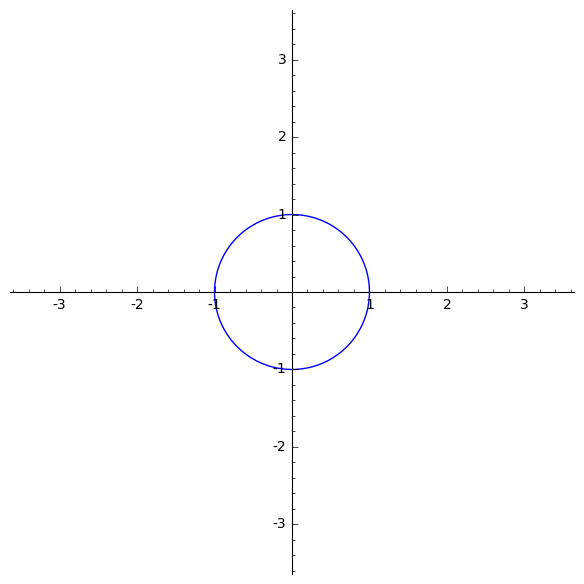
\includegraphics[width=\textwidth]{cercle.png}}\end{minipage}  & $\Rightarrow$ & \begin{minipage}{5cm}{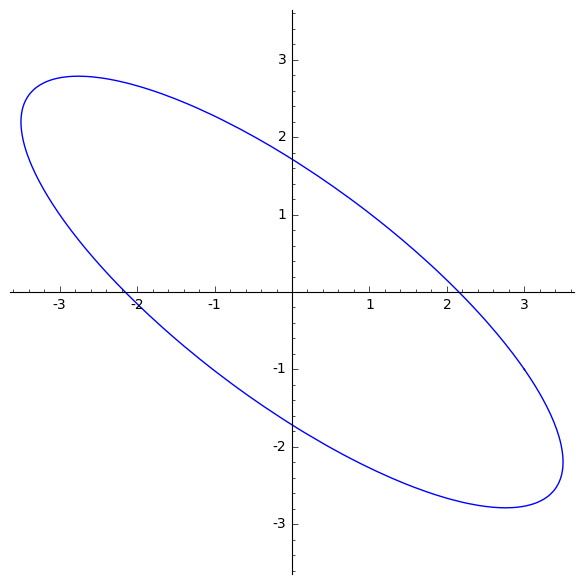
\includegraphics[width=\textwidth]{ellipse.png}}\end{minipage}
\end{tabular}}
\caption{Deformació de la circumferència unitat per l'aplicació lineal $f_A$.\label{fig:circ_ellipse}}
\end{figure}
\end{exemple}

\subsection{Classificació de formes bilineals simètriques sobre \texorpdfstring{$\mathbb{R}^n$}{Rn}}
A aquesta secció l'objectiu és classificar les formes bilineals. Definim abans què vol dir que siguin equivalents:
\begin{definicio}
Diem que dues formes bilineals $\phi_1,\phi_2\colon \K^n\times\K^n\to \K$ amb matrius corresponents $[\phi_1]$ i $\phi_2]$ \emph{són equivalents} si existeix una base $\calc$ de $\K^n$ tal que
\[
[\phi_1]=[\phi_2]_\calc .
\]
Dit d'una altra manera, si existeix una matriu invertible $\cals\in M_n(\K)$ (la matriu del canvi de base, que té per columnes els vectors de $\calc$) tal que
\[
[\phi_1]=\cals^T [\phi_2] \cals.
\]
Escriurem $q_1\sim q_2$.
\end{definicio}
\begin{lema}
Ser equivalents com a formes bilineals de $\K^n\times \K^n$ a $\K$ és una relació d'equivalència. O sigui:
\begin{itemize}
    \item $\phi \sim \phi$ per a tot $\phi$ forma bilineal (reflexiva),
    \item $\phi_1\sim \phi_2 \Leftrightarrow \phi_2 \sim \phi_1$ per a totes $\phi_1, \phi_2$ formes bilineals (simètrica) i
    \item $\phi_1\sim \phi_2$ i $\phi_2\sim \phi_3$ implica $\phi_1\sim \phi_3$ per a totes $\phi_1,\phi_2,\phi_3$ formes quadràtiques (transitiva).
\end{itemize}
\end{lema}
\begin{proof}
Cal veure en cada cas quina és la matriu $\cals$ del canvi de base:
\begin{itemize}
    \item Per veure que $\phi\sim \phi$, considerem $\cals=\1_n$,
    \item Si $\phi_1\sim \phi_2$ tenim que existeix $\cals$ una matriu de canvi de base (i per tant invertible) tal que:
    \[
    [\phi_1]=\cals^T [\phi_2] \cals.
    \]
    Però aquesta igualtat també es pot escriure com:
    \[
    [\phi_2]=(\cals^{-1})^T [\phi_1] \cals^{-1}
    \]
    i per tant $\phi_2\sim \phi_1$.
    \item Per hipòtesis tenim que existeixen $\cals_1$ i $\cals_2$ tals que:
    \[
    [\phi_1]=\cals_1^T [\phi_2] \cals_1
    \text{ i }
    [\phi_2]=\cals_2^T [\phi_3] \cals_2.
    \]
    Llavors:
    \[
    [\phi_1]=\cals_1^T \cals_2^T [\phi_3] \cals_2 \cals_1=
    (\cals_2 \cals_1)^T [\phi_3] (\cals_2 \cals_1)
    \]
    i tenim $\phi_1\sim \phi_3$.
\end{itemize}
\end{proof}

A partir d'ara considerem que $\K=\R$ i l'objectiu és classificar les formes bilineals $\phi\colon \R^n\times \R^n \to \R$:
\begin{teorema}\label{teo:class_form:bilR}
Tota forma bilineal simètrica $\phi\colon \R^n\times \R^n\to \R$ és equivalent a una forma bilineal que té per matriu una matriu diagonal amb coeficients (a la diagonal): $1$ a les $r$ primeres files, $-1$ a les $s$ següents i $0$ a les $t$ últimes ($n=r+s+t$). O sigui una matriu de la forma:
\[
\begin{pmatrix}
1      & \cdots & 0 & 0 & \cdots & 0 & 0 & \cdots & 0 \\
       & \ddots &   &   & \cdots &   &   & \cdots &  \\
0      & \cdots & 1 & 0 & \cdots & 0 & 0 & \cdots & 0 \\
0      & \cdots & 0 & -1 & \cdots & 0 & 0 & \cdots & 0 \\
       &        &   &    & \ddots &   &   & \cdots &   \\
0      & \cdots & 0 &  0 & \cdots & -1 & 0 & \cdots & 0 \\
0      & \cdots & 0 &  0 & \cdots & 0 & 0 & \cdots & 0 \\
       &        &   &    & \cdots &   &   & \ddots &   \\
0      & \cdots & 0 &  0 & \cdots & 0 & 0 & \cdots & 0 
\end{pmatrix}
\]
A més, si definim la parella $(r,s)$ com la \emph{signatura de $\phi$} ($\sign(\phi)$)\index{forma bilineal! signatura}, dues formes bilineals bilineals $\phi_1,\phi_2\colon \R^n\times \R^n\to \R$ són equivalents si i només si $\sign(\phi_1)=\sign(\phi_2)$.
\end{teorema}
\begin{proof}
Considerem $[\phi]$ la matriu simètrica $n\times n$ sobre $\R$ de la forma bilineal $\phi$. Pel Teorema espectral, existeix una matriu ortogonal $Q$  i una matriu diagonal $D$ amb valors $\lambda_1, \dots, \lambda_n$ tal que:
\[
D=Q^T [\phi] Q \,.
\]
Ara fem els canvis següents:
\begin{itemize}
    \item Podem reordenar els elements de la diagonal de $D$ reordenant les columnes de $Q$: si $Q'$ és la matriu que resulta d'intercanviar les columnes $j$ i $k$ de $Q$, llavors, $Q'$ continua sent ortogonal i el producte:
    \[
    (Q')^T[\phi]Q'
    \]
    també és diagonal, però intercanviant les posicions $i$ i $j$, o sigui, els valors $\lambda_i$ i $\lambda_j$.\\
    Aprofitem aquesta propietat per reordenar la diagonal de $D$ i posar primer els $\lambda_i>o$, llavors els $\lambda_i<0$ i finalment els $\lambda_i=0$. Per tant, podem suposar que tenim $Q$ una matriu ortogonal tal que
    \[
    D=Q^T [\phi] Q \,.
    \]
    amb $D$ una matriu diagonal tal que a la diagonal té els $r$ primers coeficients positius, els $s$ següents negatius i els $t$ últims zero.
    \item Considerem $A$ la matriu diagonal següent, definida a partir dels coeficients de $D$: el coeficient $a_{ii}$ es defineix com:
    \[
    a_{ii}=\begin{cases}
    1/\sqrt{\lambda_i} & \text{si $1\leq i \leq r$,} \\
    1/\sqrt{-\lambda_i} & \text{si $r < i \leq r+s$,} \\
    1 & \text{si $r+s < i \leq n$.}
    \end{cases}
    \]
    Tenim que $A^TDA$ és una matriu diagonal amb $r$ uns a les primeres files, $s$ menys uns a les següents i zero a les últimes.\\
    Per tant:
    \[
    [\phi] \sim A^TQ^T [\phi] QA = (QA)^T [\phi] QA
    \]
    i $(QA)^T [\phi] QA$ és diagonal i com diu l'enunciat del teorema.
\end{itemize}
De moment hem vist que, com que ser equivalent a té la propietat transitiva, si $\phi_1$ i $\phi_2$ tenen la mateixa signatura, les dues són equivalents a una mateixa forma bilineal i per tant $\phi_1\sim \phi_2$.\\
Cal veure el recíproc, o el que és equivalent, que dues matrius diagonals equivalents $D$ i $D'$ amb $(r,s,t)$ i $(r',s',t')$ coeficients $1$, $-1$ i $0$ respectivament, llavors $(r,s,t)=(r',s',t')$. \\
Com que $D$ i $D'$ són equivalents, existeix $A$ una matriu invertible que té per columnes $v_i$ tal que:
\[
D'=A^T D A.
\]
Si fem el producte de la dreta, les $r$ primeres files són $||v_1||^2$ ($D$ coincideix amb la identitat a les $r$ primeres files i columnes), \ldots, $||v_r||^2$, per tant són números positius, per tant $r'\geq r$ i argumentant canviant els papers de $D$ i $D'$ (i $A$ per $A^{-1}$), tenim $r\geq r'$, pel que $r=r'$.\\
$r+s$ és el rang de $D$. Com que $D'$ és el producte de $D$ per matrius invertibles, $r+s$ també és el rand de $D'$, que és $r'+s'$, per tant, $s=s'$.\\
Finalment, $t=n-(r+s)=n-(r'+s')=t'$.
\end{proof}
\begin{exemple}\label{exemple:class_form_bil}
Considerem la forma bilineal $\phi\colon \R^4\times\R^4\to\R$ donada per la matriu:
\[
[\phi]=\left(\begin{array}{rrrr}
1 & 5 & -1 & 3 \\
5 & 1 & 3 & -1 \\
-1 & 3 & 1 & 5 \\
3 & -1 & 5 & 1
\end{array}\right).
\]
Una manera de classificar-la és de calcular el polinomi característic i estudiar el signe dels valors on s'anul·la:
\[
p_{[\phi]}(x)=\det(A-x\1_4)=x^{4} - 4 x^{3} - 64 x^{2} + 256 x .
\]
I $p_{[\phi]}(x)$ s'anul·la als valors $\{-8,0,4,8\}$, per tant té signatura $(2,1)$ i és equivalent a la forma bilineal que té per matriu:
\[
\begin{pmatrix} 1 & 0 & 0 & 0 \\ 0 & 1 & 0 & 0 \\ 0 & 0 & -1 & 0 \\ 0 & 0 & 0 & 0 \end{pmatrix} .
\]
\end{exemple}

Acabem aquesta secció aprofitant aquesta classificació per fer la corresponent de les formes quadràtiques.

\begin{definicio}
Una \emph{forma quadràtica}\index{forma quadràtica} sobre un cos $\K$ és una aplicació $q\colon \K^n\to \K$ que es pot expressar com:
\[
q(x_1, \dots , x_n)=\sum_{1\leq i , j \leq n} \lambda_{ij}x_i x_j
\]
amb $\lambda_{ij}\in \K$.

També es pot escriure com:
\[
q(x_1, \dots , x_n)= \vec x^T A \vec x ,
\]
on $\vec x=\smat{x_1 \\ \vdots \\ x_n}$ i $A$ és la matriu (simètrica) que té per coeficients
\[
a_{ij}=\begin{cases} \lambda_{ii} & \text{si $i=j$,} \\ \frac{\lambda_{ij}+\lambda_{ji}}{2} & \text{si $i\neq j$.}\end{cases}
\]
\end{definicio}

\begin{observacio}
Amb el que hem vist, tenim una bijecció entre les matrius simètriques (que es poden pensar com formes bilineals en una base donada) i les formes quadràtiques. Escriurem $[q]$ per denotar la matriu simètrica corresponent a la forma quadràtica $q$.
\end{observacio}
\begin{exemple}
La forma quadràtica $q\colon \R^2 \to \R$ definida per $q(x_1,x_2)=ax_1^2+bx_1x_2+cx_2^2$ correspon a la matriu simètrica
\[
\begin{pmatrix}
a & b/2 \\ b/2 & c
\end{pmatrix} .
\]
Podem recuperar la forma quadràtica fent:
\[
q(x_1,x_2)=\begin{pmatrix} x_1 & x_2 \end{pmatrix}\begin{pmatrix}
a & b/2 \\ b/2 & c
\end{pmatrix} \begin{pmatrix} x_1 \\ x_2 \end{pmatrix}=ax_1^2 + bx_1x_2+cx_2^2 .
\]
\end{exemple}
\begin{exemple}
Considerem les formes quadràtiques $q_1$ i $q_2$ de $\R^2$ a $\R$ definides com $q_1(x_1,x_2)=x_1x_2$ i $q_2(y_1,y_2)=y_1^2-y_2^2$. Observem que si fem el canvi de base:
\[
\begin{pmatrix} y_1 \\ y_2  \end{pmatrix} =
\begin{pmatrix} 1/2 & 1/2 \\ 1/2 & -1/2 \end{pmatrix}
\begin{pmatrix} x_1 \\ x_2  \end{pmatrix}
\]
es poden escriure:
\[
y_1=\frac12x_1+\frac12x_2 \text{ i } y_2=\frac12x_1-\frac12x_2 
\]
i tenim
\[
q_2(y_1,y_2)=(\frac12x_1+\frac12x_2)^2 - (\frac12x_1-\frac12x_2)^2=x_1x_2 .
\]
Per tant, tenen la mateixa forma. Aquesta igualtat també es pot veure en forma matricial observant que si $\cals$ és la matriu del canvi de base, tenim $[q_1]=\cals^T [q_2] \cals$, on $[q_1]$ i $[q_2]$ són les matrius simètriques corresponents a les formes bilineals $q_1$ i $q_2$ respectivament:
\[
\begin{pmatrix} 0 & 1/2 \\ 1/2 & 0 \end{pmatrix}=
\begin{pmatrix} 1/2 & 1/2 \\ 1/2 & -1/2 \end{pmatrix}^T
\begin{pmatrix} 1 & 0 \\ 0 & -1 \end{pmatrix}
\begin{pmatrix} 1/2 & 1/2 \\ 1/2 & -1/2 \end{pmatrix}
\]
\end{exemple}
\begin{definicio}
Diem que dues formes quadràtiques $q_1,q_2\colon \K^n\to \K$ \emph{són equivalents}, amb matrius  si existeix un canvi de base $\cals$ a $\K^n$ tal que 
\[
[q_1]=\cals^T [q_2] \cals.
\]
Escriurem $q_1\sim q_2$.
\end{definicio}

Com que els canvis de base afecten de la mateixa manera que afectaven a les formes bilineals (veure Lema \ref{lema:canvi_base_forma_bil}), obtenim que ``\emph{ser equivalent a}'' també es una relació d'equivalència a les formes quadràtiques i l'anàleg al Teorema \ref{teo:class_form:bilR}:
\begin{teorema}\label{teo:class_formQuadR}
Tota forma quadràtica $q\colon \R^n\to \R$ és equivalent a una forma bilineal del tipus:
\[
q_1(x_1,\dots, x_n)=x_1^2+ \cdots + x_r^2 - x_{r+1}^2-\cdots -x_{r+s}^2 .
\]
A més, si definim la parella $(r,s)$ com la \emph{signatura de $q$} ($\sign(q)$)\index{forma quadràtica! signatura}, dues formes quadràtiques $q_1,q_2\colon \R^n\to \R$ són equivalents si i només si $\sign(q_1)=\sign(q_2)$.
\end{teorema}
\begin{exemple}
Classifiquem la forma quadràtica $q\colon \R^4 \to \R$:
\[
q(x_1,x_2,x_3,x_4)=x_1^2+10 x_1x_2 -2 x_1x_3+6x_1x_4 + x_2^2 -6x_2x_3-2x_2x_4+x_3^3+10x_3x_4-x_4^2.
\]
Que té per matriu:
\[
\left(\begin{array}{rrrr}
1 & 5 & -1 & 3 \\
5 & 1 & 3 & -1 \\
-1 & 3 & 1 & 5 \\
3 & -1 & 5 & 1
\end{array}\right)
\]
Per tant, podem aprofitar els càlculs de l'Exemple \ref{exemple:class_form_bil}, i tenim que és equivalent a:
\[
q(y_1,y_2,y_3,y_4)=y_1^2+y_2^2-y_3^2.
\]
\end{exemple}

\begin{llista-exercicis}
\item[Secció 5.1:] 12, 16, 18.
\item[Secció 5.2:] 14, 34, 38.
\item[Secció 5.3:] 5-11, 13-20, 32.
\item[Secció 5.4:] 2, 8, 10.
\item[Secció 5.5:] 4, 10, 16, 22.
\item[Secció 8.1:] 6, 12, 16, 22.
\item[Secció 8.2:] 4, 10, 18, 22.
\item[Secció 8.3:] 6, 16, 18, 20.
\end{llista-exercicis}